\pagestyle{fancy}
\fancyhf{}
\fancyhead[R]{\texttt{kvant.mccme.ru}}
\renewcommand{\headrulewidth}{0pt}
\begin{center}
    {\LARGE\bfseries 39}
    \vspace{-0.5em}
    \rule{\textwidth}{0.2pt}
    {\textbf {задачник кванта}}
\end{center}




\begin{multicols}{2}

    \begin{center}
        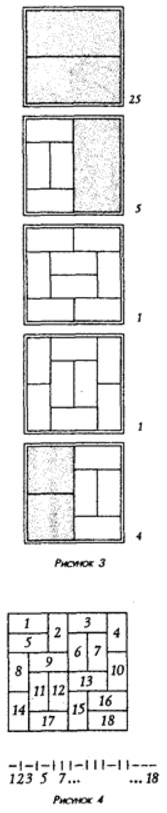
\includegraphics[height=16cm, width=4.5cm]{/home/cun/Documents/LatexLab/photos/photo_2024-12-03_02-54-18.jpg}
    \end{center}
\raggedleft
\textbf{Ф1368}. Велосипедное колесо радиусом \(R = 50cm\) немного деформировали
-оно осталось полоским, но превратилось в эллипс с разностью полуоссей \(\Theta = a - b = 1cm\).
При какой скорости качения этого колеса по горизонтальной поверхности оно начнёт подпрыгивать?

\columnbreak
\raggedright
.

\end{multicols}